\documentclass[xcolor=table]{beamer}

\usepackage[french]{babel}
\usepackage[latin1]{inputenc}
\usepackage[normalem]{ulem}
\usepackage[T1]{fontenc}
\usepackage{fancyhdr}   %% Pour la gestion des num�ros de page
\usepackage{graphicx}
\usepackage{amsmath}
\usepackage{mathrsfs}
\usepackage{amsfonts}
\usepackage{palatino}        %% Palatino fonts
\usepackage{mathptm}        %% PostScript Type 1 math fonts
\usepackage{dsfont} %% Pour mathds
\usepackage{color}
%%\usepackage{pstricks}
\usepackage{xmpmulti}
\usepackage{hyperref}
\usepackage{multimedia}
\usepackage{multirow}
%\usepackage[table]{xcolor}
\usepackage{fourier-orns}
\usepackage{subfigure}
\usepackage{tikz}

\DeclareMathAlphabet{\mathpzc}{OT1}{pzc}{m}{it}

\definecolor{vert}{rgb}{0.07,0.7,0.00}
\definecolor{gris}{gray}{0.70}
\definecolor{gris2}{gray}{0.95}
\definecolor{bleu}{rgb}{0.19,0.19,0.68}

%table setting
\newcommand\T{\rule{0pt}{2.6ex}}
\newcommand\B{\rule[-1.2ex]{0pt}{0pt}}
\renewcommand{\thesubfigure}{\thefigure.\arabic{subfigure}}

\usetheme{allee_marine} %voir fichier beaerthemeallee_marine.sty   ==> \usetheme{allee_marine}


%%%%%%%%%%%%%%%%%%%%%%%%%% Pr�sentation du document %%%%%%%%%%%%%%%%%%%%%%%%%%
\title[Master 1 Project]{Indexing big colored image bank : Texture 3.0}
\author[Etienne CAILLAUD, Thomas LE BRIS, Ibrahima GUEYE, Gaetan ADIER]{\textbf{Etienne CAILLAUD, Thomas LE BRIS, Ibrahima GUEYE, Gaetan ADIER}}
\institute [XLIM-SIC UMR CNRS 7252]{\textbf{XLIM-SIC Laboratory UMR CNRS 7252, Poitiers, France}}
\date{}

%%%%%%%%%%%%%%%%%%%%%%% Num�ro de pages en bas � gauche %%%%%%%%%%%%%%%%%%%%%%
\addtobeamertemplate{footline}{\color{vert}\hfill\insertframenumber/\inserttotalframenumber}

\pgfdeclareimage[height=96mm,width=128mm]{nombidon}{Fond}
\setbeamertemplate{background}{\pgfuseimage{nombidon}}

\pgfdeclareimage[height=96mm,width=128mm]{nombidon2}{Fond1}
\setbeamertemplate{background}{\pgfuseimage{nombidon2}}

%%----------------------------------------------------------------------------
%% A chaque d�but de sous-section : g�n�re une table des mati�res
%%----------------------------------------------------------------------------
\AtBeginSection[]
{
   \setbeamertemplate{background}{\pgfuseimage{nombidon}}
   \begin{frame}<beamer>
    \frametitle{Outline}
    \tableofcontents[currentsection, hideallsubsections] %% affiche la section courante et les autres en gris�, masque les sous-sections
   \end{frame}
  \setbeamertemplate{background}{\pgfuseimage{nombidon2}}
}

\AtBeginSubsection[]
{
  \setbeamertemplate{background}{\pgfuseimage{nombidon}}
  \begin{frame}<beamer>
    \tableofcontents[sectionstyle=show/shaded,subsectionstyle=show/shaded/hide, subsubsectionstyle =hide]
  \end{frame}
   \setbeamertemplate{background}{\pgfuseimage{nombidon2}}
}

\AtBeginSubsubsection[]
{
  \setbeamertemplate{background}{\pgfuseimage{nombidon}}
  \begin{frame}<beamer>
    \tableofcontents[sectionstyle=show/shaded,subsectionstyle=show/shaded/hide,subsubsectionstyle =show/shaded/hide]
  \end{frame}
   \setbeamertemplate{background}{\pgfuseimage{nombidon2}}
}


%%%%%%%%%%%%%%%%%%%%%%%%%%%%%%%%%%%%%%%%%%%%%%%%%%%%%%%%%%%%%%%%%%%%%%%%%%%%%%
%%%%%%%%%%%%%%%%%%%%%%%%%%%%                       %%%%%%%%%%%%%%%%%%%%%%%%%%%
%%%%%%%%%%%%%%%%%%%%%%%%%%     D�BUT DU DOCUMENT     %%%%%%%%%%%%%%%%%%%%%%%%%
%%%%%%%%%%%%%%%%%%%%%%%%%%%%                       %%%%%%%%%%%%%%%%%%%%%%%%%%%
%%%%%%%%%%%%%%%%%%%%%%%%%%%%%%%%%%%%%%%%%%%%%%%%%%%%%%%%%%%%%%%%%%%%%%%%%%%%%%
\begin{document}
\graphicspath{{images/}}
\setbeamercolor{block title example}{bg = gray}

\begin{frame}
    \vspace{-1.5cm}
    \begin{tikzpicture}[remember picture,overlay]
        \node[xshift=0cm, above=8.6cm] at (current page.south west)
        {
\includegraphics[width=40cm,height=0.9cm]{cache_titre.png}};
        \node[xshift=2cm, above=2.8cm] at (current page.south west)
        {
\includegraphics[height=1.5cm]{Xlim.png}};
        \node[xshift=11cm, above=3cm] at (current page.south west)
        {
\includegraphics[height=1cm]{logo_une.jpg}};
        \node[xshift=6.5cm, above=0.7cm] at (current page.south west)
        {
\includegraphics[height=1.6cm]{Lifeclef.png}};
    \end{tikzpicture}
    \titlepage
\end{frame}

%%%%%%%%%%%%%%%%%%%%%%%%%%%%%%%%%%%%%%%%%%%%%%%%%%%%%%%%%%%%%%%%%%%%%%%%%%%%%%%%%%%%%%%%%%%%%%%%%%%%%
%%%%%%%%%%%                        D�but de la pr�sentation                       			 %%%%%%%%
%%%%%%%%%%%%%%%%%%%%%%%%%%%%%%%%%%%%%%%%%%%%%%%%%%%%%%%%%%%%%%%%%%%%%%%%%%%%%%%%%%%%%%%%%%%%%%%%%%%%%
\section{Introduction to the project context}
%%-----------------------------------------------------------------------------------------
%%-----------------------------------------------------------------------------------------
\begin{frame} \frametitle{Project context (1/2)}
%%-----------------------------------------------------------------------------------------
%% objective + image index
%%-----------------------------------------------------------------------------------------

\begin{block}{What is a imageCLEF ?}
    International contest which purpose is to benchmark plant identification from images.
\end{block}

	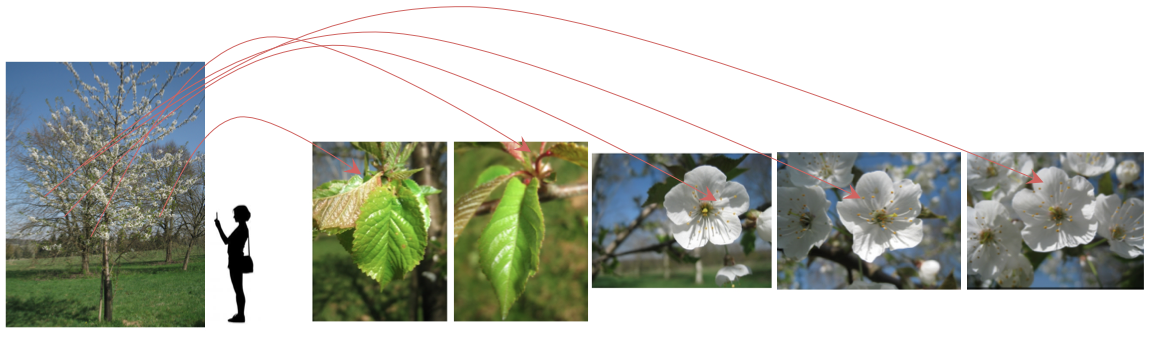
\includegraphics[scale=0.27]{OnePrunus.png}



\end{frame}
%%-----------------------------------------------------------------------------------------

\begin{frame} \frametitle{Project context 2/2}
%----------------------------------------------------------------------------------------
%%User requirement
%----------------------------------------------------------------------------------------
\begin{columns}[t]
  \begin{column}{5cm}
  \begin{block}{Objectives}

    \begin{itemize}
        \item Adapt XLIM's descriptor to image classification
        \item Benchmark results
    \end{itemize}
\end{block}
  \end{column}

  \begin{column}{5cm}
 \begin{alertblock}{Constraints}
    \begin{itemize}
        \item Use of Python language
        \item Parallel programming
    \end{itemize}
\end{alertblock}
  \end{column}
\end{columns}

\begin{figure}
    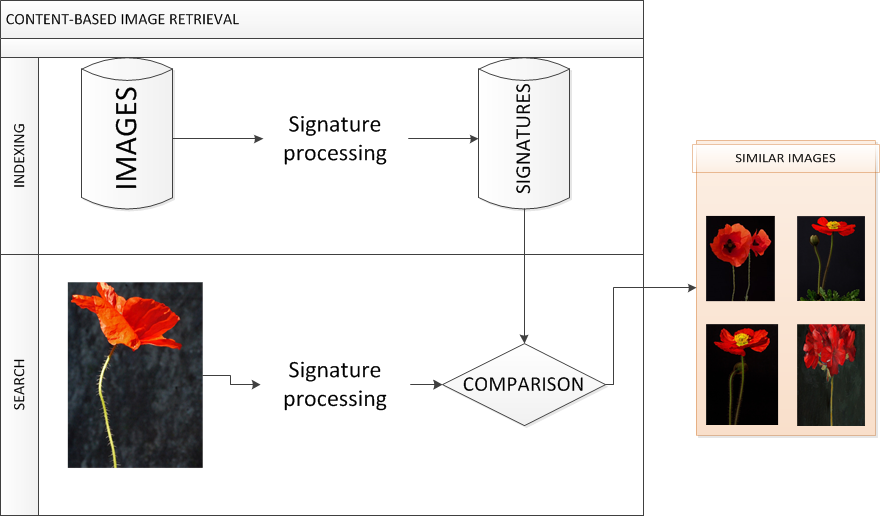
\includegraphics[scale=0.34]{CBIR.png}
\end{figure}

\end{frame}
%%-----------------------------------------------------------------------------------------


%%-----------------------------------------------------------------------------------------
%%-----------------------------------------------------------------------------------------

\begin{frame} \frametitle{Team presentation}
%%-----------------------------------------------------------------------------------------

% Schema demande par mr Richard
\begin{figure}[h]
    \center
    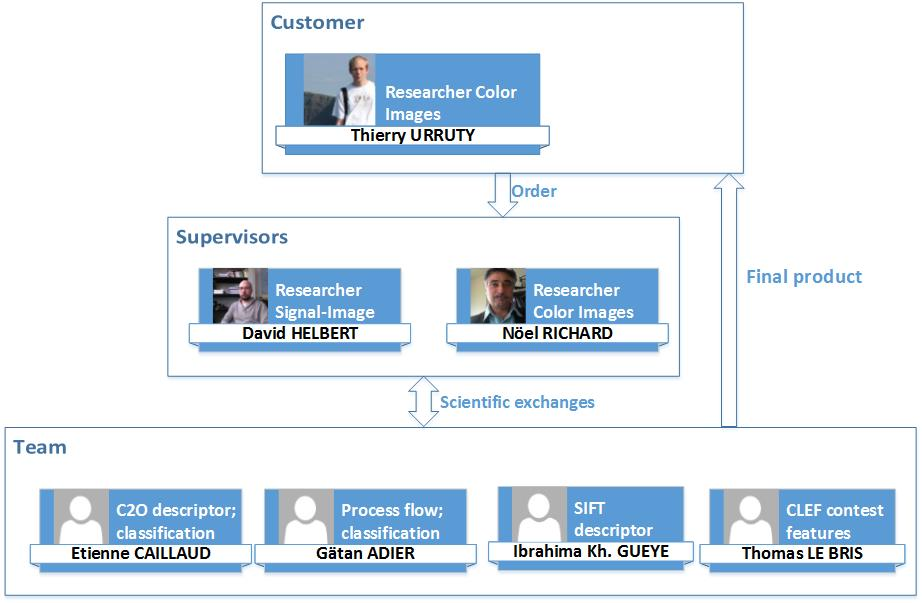
\includegraphics[scale=0.45]{Dessin1.jpg}
    \caption{Team}\label{fig:team}
\end{figure}

\end{frame}
%%-----------------------------------------------------------------------------------------

% A INCLURE CLAIREMENT DANS L'INTRODUCTION
%\begin{frame} \frametitle{User requirement}
%%-----------------------------------------------------------------------------------------

% Parler de la demande de base, ce qui etait convenu avec le client ...

%\begin{itemize}
% \item Design  software programs:\\
%   indexation of  images database,calculate descriptor according to  nature images
%\item Adapt the last up to date designed color and texture attributes to the current image classification
%\item Compare our results (using CLEF challenge metrics)
%\item Provide an abstract of the comparisons and a technical report
%\end{itemize}

%\end{frame}
%%-----------------------------------------------------------------------------------------


\section{Work and results}
\begin{frame} \frametitle{SIFT descriptor(1/2)}

\begin{tikzpicture}[remember picture, overlay]
  \node [anchor=north east, inner sep=2pt]  at (current page.north east)
     {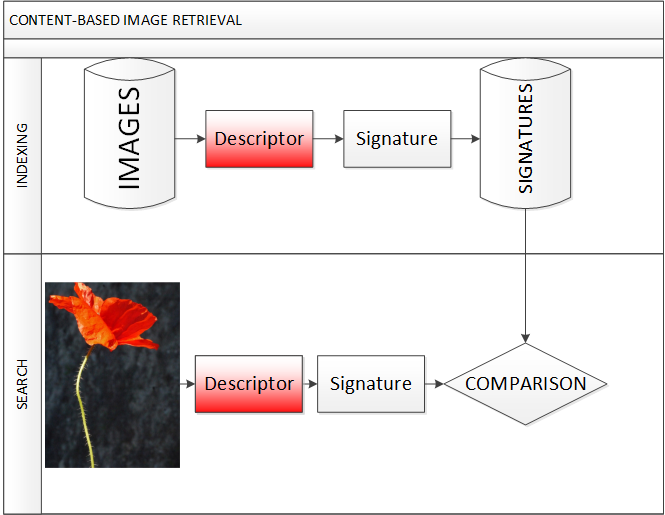
\includegraphics[height=2.5cm]{DescriptorTopImg.png}};
\end{tikzpicture}

Key-points detection (x,y,$\sigma$)


\begin{figure}[htbp]
    \begin{minipage}[c]{.45\linewidth}
      \begin{itemize}

    \item Scale-space extrema detection\\


    \item  Key-point location\\


    \item Orientation assignment\\


    \item Key-point descriptor

    \end{itemize}
    \end{minipage}
    \hfill
    \begin{minipage}[c]{.45\linewidth}
      \begin{center}
	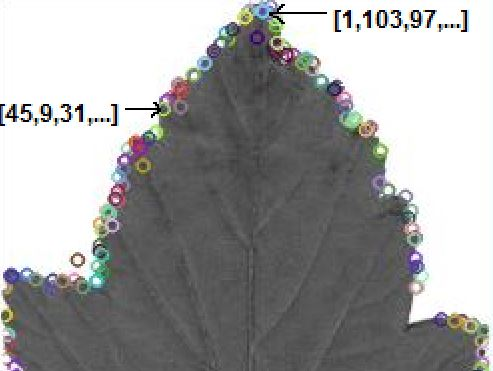
\includegraphics[scale=0.45]{siftKP2.jpg}
	\caption{SIFT Keypoints}
	\label{figure:Illustration}
      \end{center}
    \end{minipage}
  \end{figure}





\end{frame}

\begin{frame} \frametitle{SIFT descriptor(2/2)}
% Image en haut a droite rapellant l'avancee dans le process flow
\begin{tikzpicture}[remember picture, overlay]
  \node [anchor=north east, inner sep=2pt]  at (current page.north east)
     {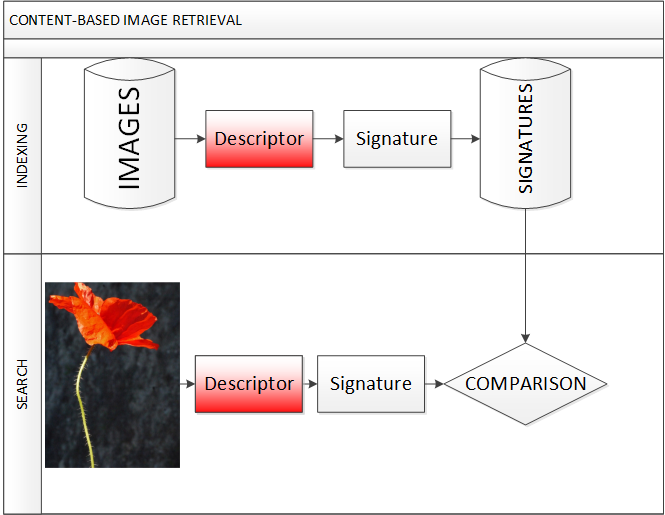
\includegraphics[height=2.5cm]{DescriptorTopImg.png}};
\end{tikzpicture}

\begin{figure}[htbp]
    \begin{minipage}[c]{.45\linewidth}
      \begin{center}
	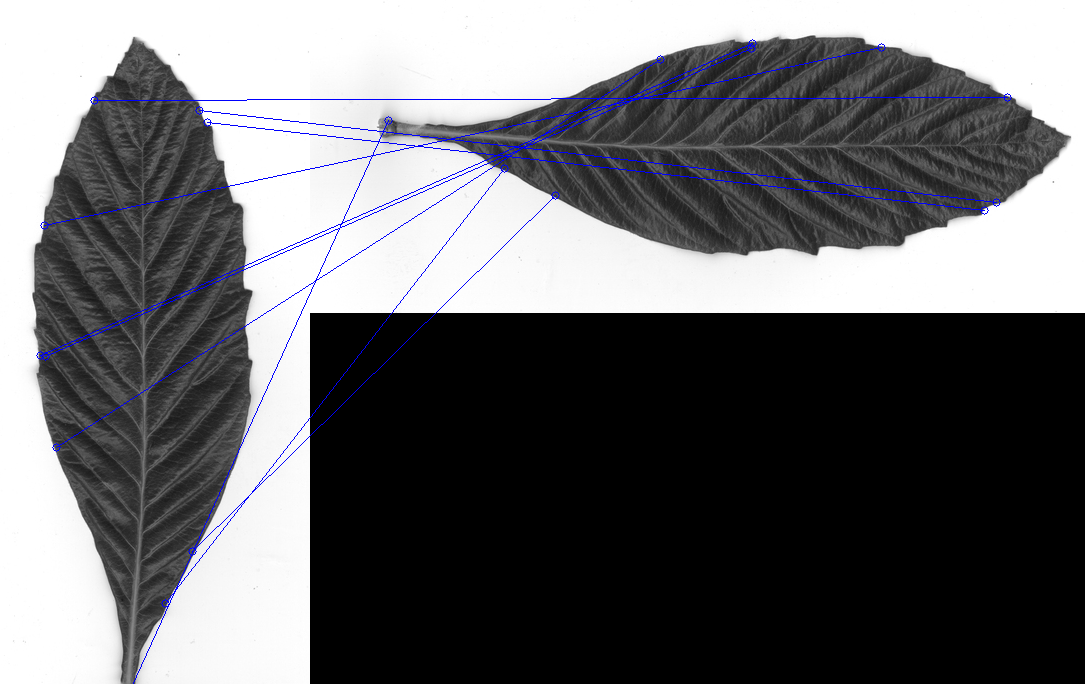
\includegraphics[scale=0.20]{Capture1.png}
	\caption{SIFT Matching for rotation}
	\label{figure:Illustration}
      \end{center}
    \end{minipage}
    \hfill
    \begin{minipage}[c]{.45\linewidth}
      \begin{center}
	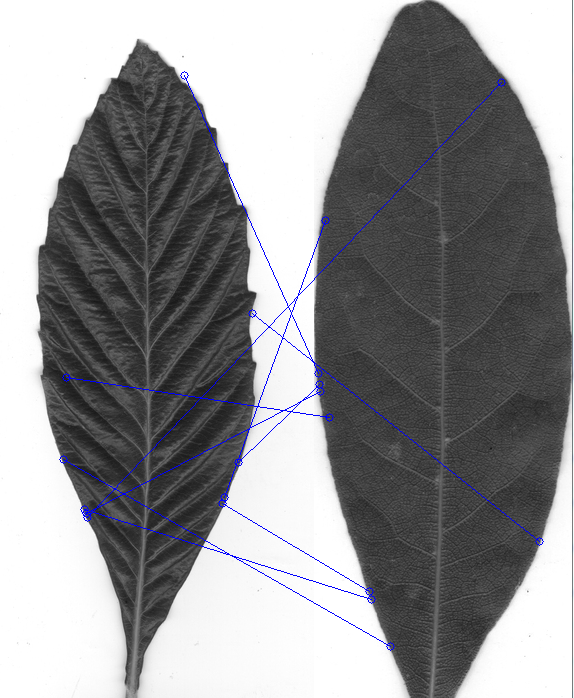
\includegraphics[scale=0.20]{Capture.png}
	\caption{SIFT matching for scale changes}
	\label{figure:Illustration}
      \end{center}
    \end{minipage}
  \end{figure}
\end{frame}



\begin{frame} \frametitle{What about nature images?}
%%-----------------------------------------------------------------------------------------
% Commencer par l'interet des C2O par rapport aux autres descripteurs, (difference entre traitement vectoriel et marginal,...)

% Image en haut a droite rapellant l'avancee dans le process flow
\begin{tikzpicture}[remember picture, overlay]
  \node [anchor=north east, inner sep=2pt]  at (current page.north east)
     {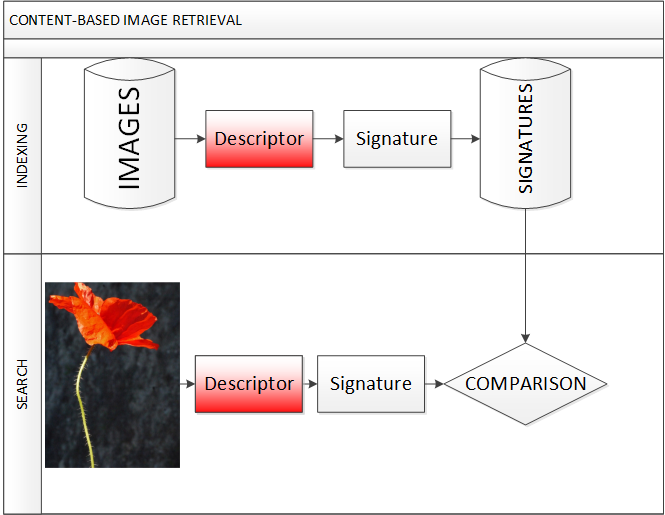
\includegraphics[height=2.5cm]{DescriptorTopImg.png}};
\end{tikzpicture}

\begin{columns}[t]
  \begin{column}{5cm}
  \begin{block}{SIFT descriptor}
	\begin{itemize}
		\item Description using orientation of shapes
		\item Natively used on grayscale images
		\item Only marginal methods for color images
		\item Unable to get the texture information from image
	\end{itemize}
  \end{block}
  \end{column}

  \begin{column}{5cm}
  \begin{block}{C$_2$O descriptor}
  \begin{itemize}
		\item Description based on color difference
		\item Natively conceived for color images
		\item Take account of the texture information
  \end{itemize}
  \end{block}
  \end{column}
 \end{columns}
\end{frame}
%%-----------------------------------------------------------------------------------------






\begin{frame} \frametitle{C$_2$O descriptor (1/2)}
%%-----------------------------------------------------------------------------------------

% Image en haut a droite rapellant l'avancee dans le process flow
\begin{tikzpicture}[remember picture, overlay]
  \node [anchor=north east, inner sep=2pt]  at (current page.north east)
     {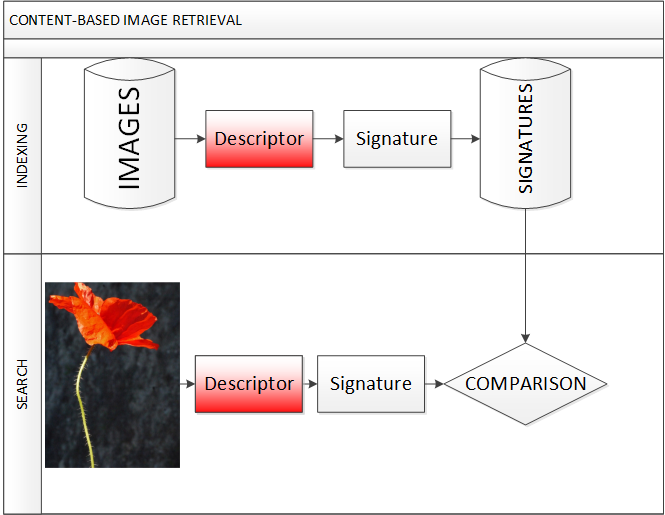
\includegraphics[height=2.5cm]{DescriptorTopImg.png}};
\end{tikzpicture}

% Mettre des exemples de matrice C2O sur des images de la base qui seront parlant !!

\begin{itemize}


\item<1-> The C$_2$O matrix for a poorly textured image :
\only<1> {\begin{figure}[htbp]
    \begin{minipage}[c]{.40\linewidth}
      \begin{center}
    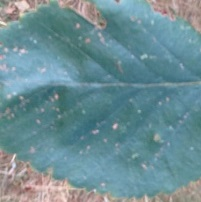
\includegraphics[scale=1.0]{61p.jpg}
    \caption{Image to characterize}
    \label{fig:Sig}
      \end{center}
    \end{minipage}
    \hfill
    \begin{minipage}[c]{.55\linewidth}
      \begin{center}
    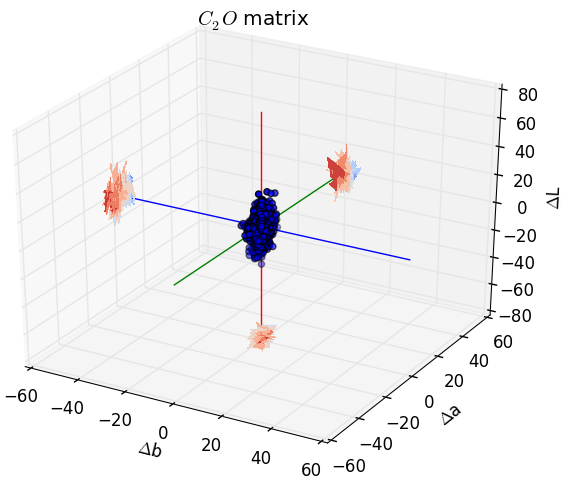
\includegraphics[scale=0.38]{C2OMat61p.png}
    \caption{Signature}
    \label{fig:Sig}
      \end{center}
    \end{minipage}
\end{figure}}
\item<2-> The C$_2$O matrix for a more textured and colored image :
\only<2> {\begin{figure}[htbp]
    \begin{minipage}[c]{.40\linewidth}
      \begin{center}
    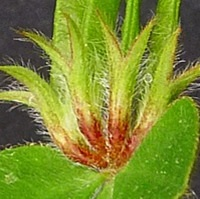
\includegraphics[scale=0.50]{97p.jpg}
    \caption{Image to characterize}
    \label{fig:Sig}
      \end{center}
    \end{minipage}
    \hfill
    \begin{minipage}[c]{.55\linewidth}
      \begin{center}
    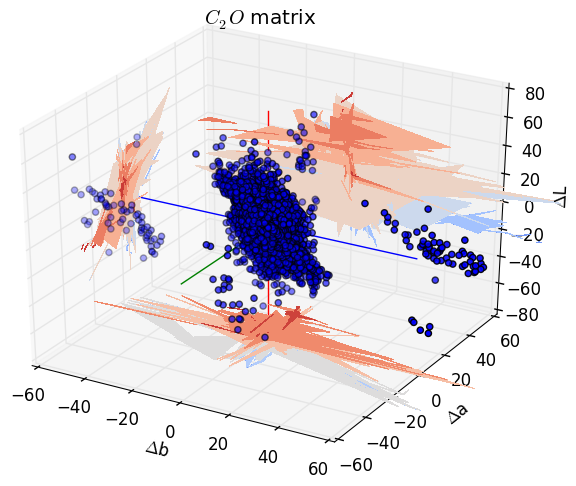
\includegraphics[scale=0.38]{C2OMat97p.png}
    \caption{Signature}
    \label{fig:Sig}
      \end{center}
    \end{minipage}
\end{figure}}

\end{itemize}

\end{frame}
%%-----------------------------------------------------------------------------------------


\begin{frame} \frametitle{C$_2$O descriptor (2/2)}
%%-----------------------------------------------------------------------------------------

% Mettre en petit en haut l'illustration coords spheriques et montrer les signatures correspondant aux matrices


% Image en haut a droite rapellant l'avancee dans le process flow
\begin{tikzpicture}[remember picture, overlay]
  \node [anchor=north east, inner sep=2pt]  at (current page.north east)
     {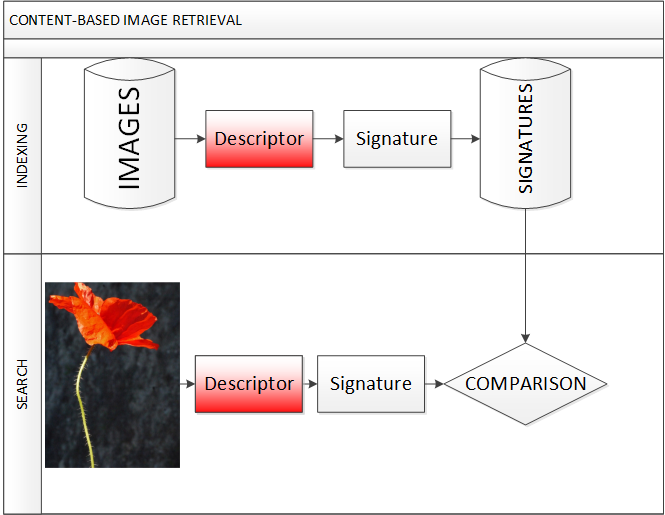
\includegraphics[height=2.5cm]{DescriptorTopImg.png}};
\end{tikzpicture}


\begin{tikzpicture}[remember picture, overlay]
  \node [anchor=south east, inner sep=20pt]  at (current page.south east)
     {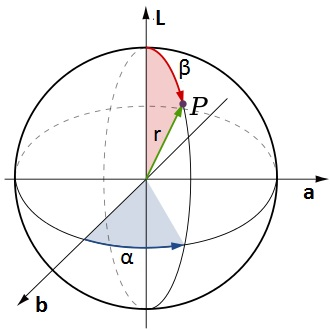
\includegraphics[height=3.5cm]{Spherical_Coordinates}};
\end{tikzpicture}

% Montrer la transition matrice - signature
\begin{tikzpicture}[remember picture, overlay]
  \node [anchor=north west, inner sep=50pt]  at (current page.north west)
     {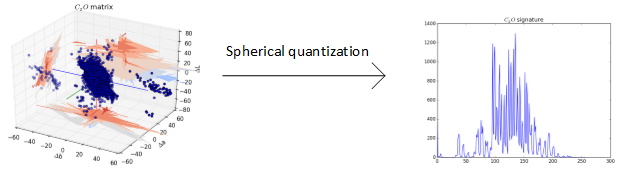
\includegraphics[height=1.5cm]{matrixtosig.png}};
\end{tikzpicture}

\begin{itemize}
\item<1-> The C$_2$O signature for a poorly textured image :
\only<1> {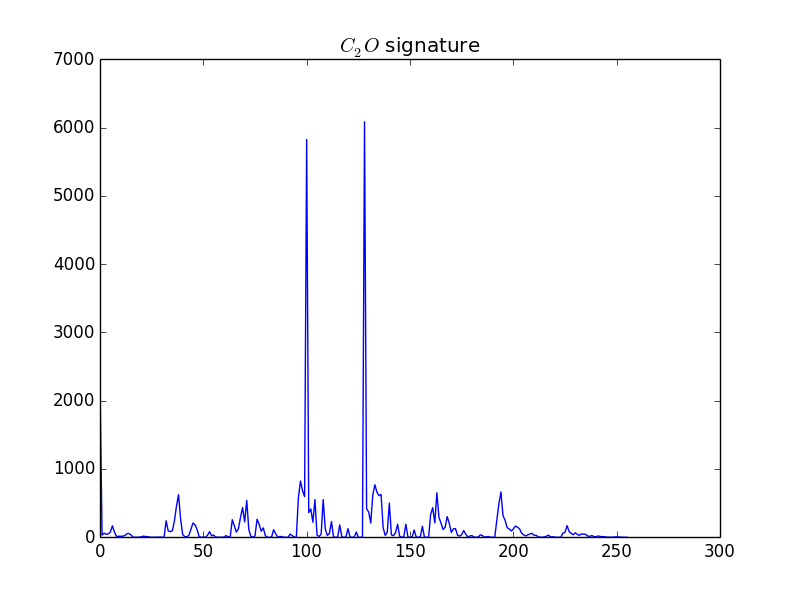
\includegraphics[height=4cm]{C2OSig61p.png}}
\item<2-> The C$_2$O signature for a more textured and colored image :
\only<2> {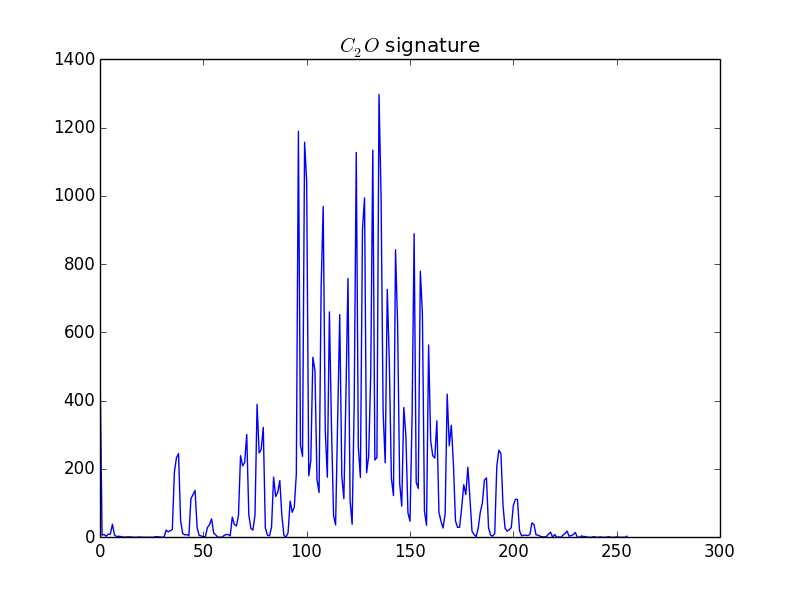
\includegraphics[height=4cm]{C2OSig97p.png}}

\end{itemize}




\end{frame}
%%-----------------------------------------------------------------------------------------



\begin{frame} \frametitle{Bag of word (1/2)}
%----------------------------------------------------------------------------------------

% Image en haut a droite rapellant l'avancee dans le process flow
\begin{tikzpicture}[remember picture, overlay]
\node [anchor=north east, inner sep=2pt] at (current page.north east)
{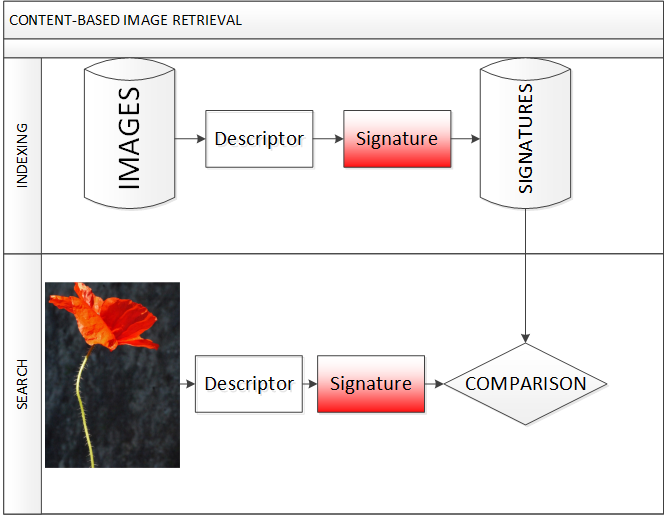
\includegraphics[height=2.5cm]{SignatureTopImg.png}};
\end{tikzpicture}

Reducing the number of points (100 in our case).

\begin{itemize}
\item K-means
\begin{itemize}
\item Attribute the vectors to centroid vectors.
\end{itemize}
\end{itemize}

\begin{figure}[htbp]
\begin{minipage}[c]{.4\linewidth}
\begin{center}
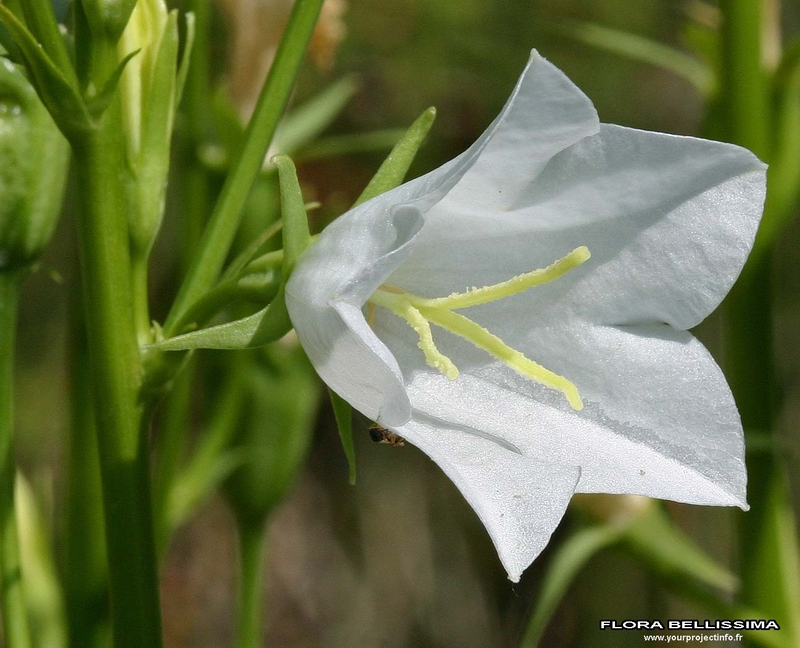
\includegraphics[scale=0.10]{87.jpg}
\label{fig:image4}
\end{center}
\end{minipage}
\hfill
\begin{minipage}[c]{.5\linewidth}
\begin{center}
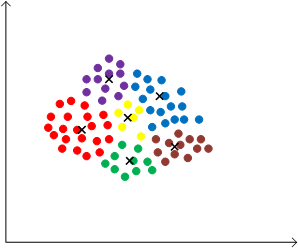
\includegraphics[scale=0.35]{kmeans_img_1.png}
\label{fig:image5}
\end{center}
\end{minipage}
\end{figure}


\begin{figure}[htbp]
\begin{minipage}[c]{.4\linewidth}
\begin{center}
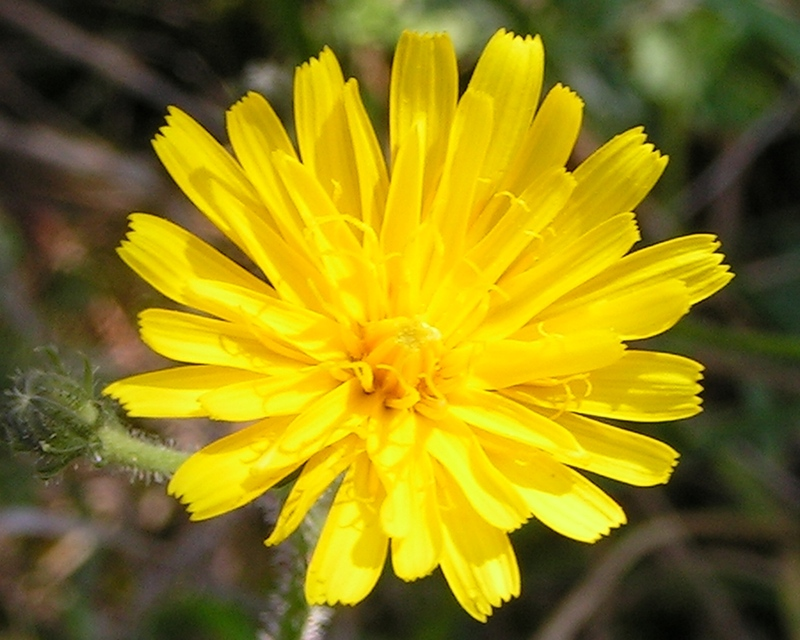
\includegraphics[scale=0.10]{21604.jpg}
\label{fig:image6}
\end{center}
\end{minipage}
\hfill
\begin{minipage}[c]{.5\linewidth}
\begin{center}
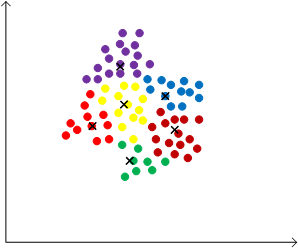
\includegraphics[scale=0.35]{kmeans_img_2.png}
\label{fig:image7}
\end{center}
\end{minipage}
\end{figure}

\end{frame}
%----------------------------------------------------------------------------------------

\begin{frame} \frametitle{Bag of word (2/2)}
%----------------------------------------------------------------------------------------

% Image en haut a droite rapellant l'avancee dans le process flow
\begin{tikzpicture}[remember picture, overlay]
\node [anchor=north east, inner sep=2pt] at (current page.north east)
{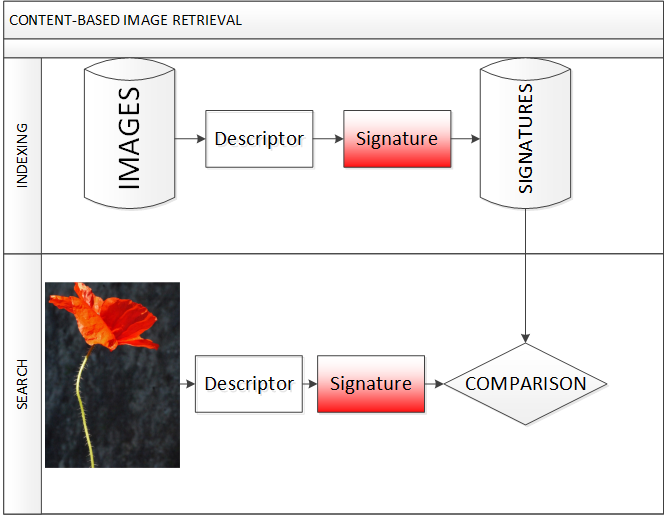
\includegraphics[height=2.5cm]{SignatureTopImg.png}};
\end{tikzpicture}

\begin{itemize}
\item Signature
\begin{itemize}
\item Design histogram in function of assignment of the vectors.
\end{itemize}
\end{itemize}

\begin{figure}[htbp]
\begin{minipage}[c]{.45\linewidth}
\begin{center}
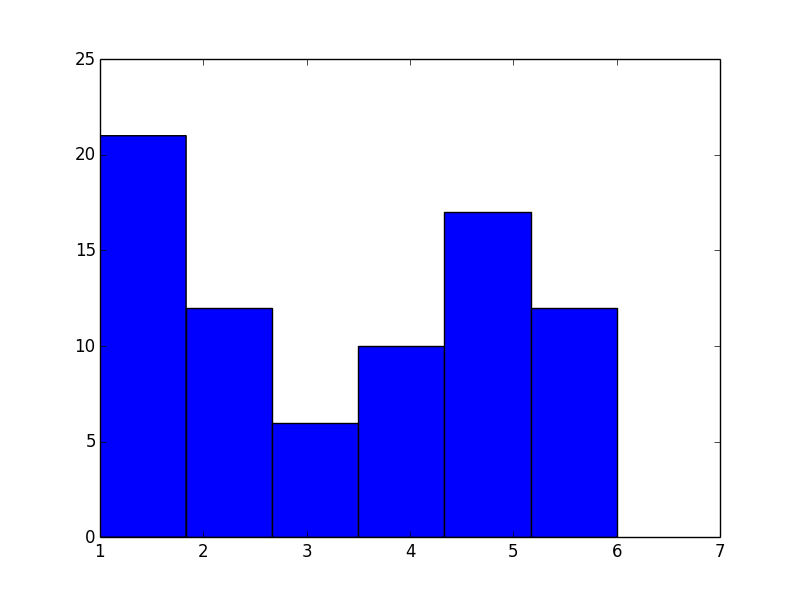
\includegraphics[scale=0.20]{hist_img_1.png}
\caption{image 1}
\label{fig:image4}
\end{center}
\end{minipage}
\hfill
\begin{minipage}[c]{.45\linewidth}
\begin{center}
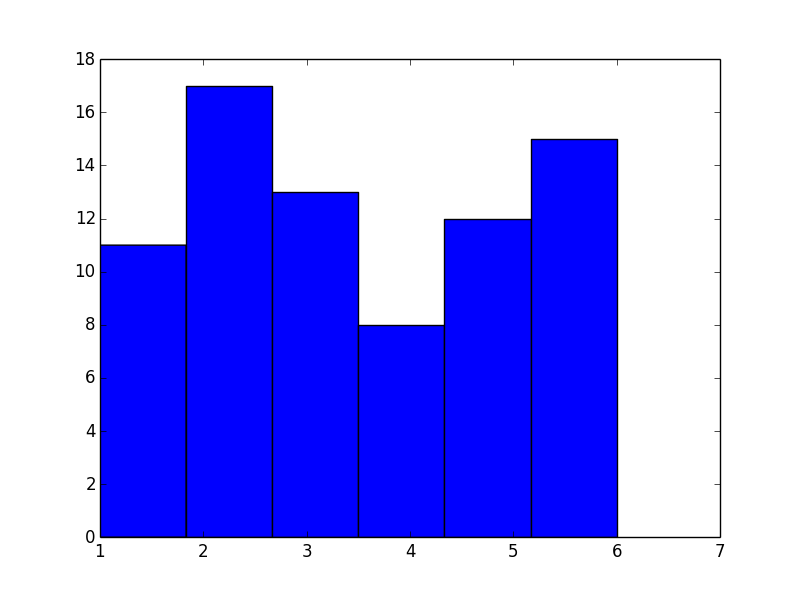
\includegraphics[scale=0.20]{hist_img_2.png}
\caption{image 2}
\label{fig:image5}
\end{center}
\end{minipage}
\end{figure}


\end{frame}
%----------------------------------------------------------------------------------------


\begin{frame}\frametitle{K-nn(1/2)}

% Image en haut a droite rapellant l'avancee dans le process flow
\begin{tikzpicture}[remember picture, overlay]
  \node [anchor=north east, inner sep=2pt]  at (current page.north east)
     {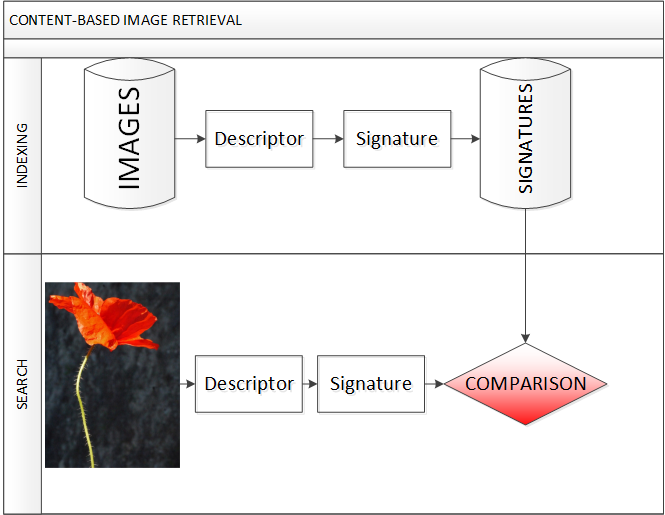
\includegraphics[height=2.5cm]{knnTopImg.png}};
\end{tikzpicture}

- The k nearest neighbor method

\begin{itemize}
\item<1-> Comparison to the dictionary .
\only<1> {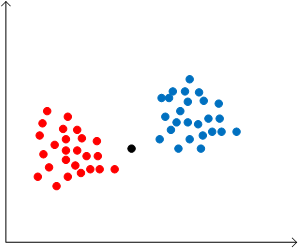
\includegraphics[height=4.2cm]{knnwc.png}} % Changer l'image
\only<2> {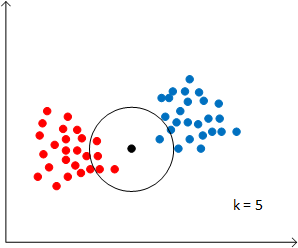
\includegraphics[height=4cm]{knnac.png}
\item 4 occurrences of {the \color{red} red} class
\item 1 occurrence of {the \color{blue} blue} class
\item The new point is attributed to {the \color{red} red} class}
\end{itemize}

\end{frame}

\begin{frame}\frametitle{K-nn(2/2)}

% Image en haut a droite rapellant l'avancee dans le process flow
\begin{tikzpicture}[remember picture, overlay]
  \node [anchor=north east, inner sep=2pt]  at (current page.north east)
     {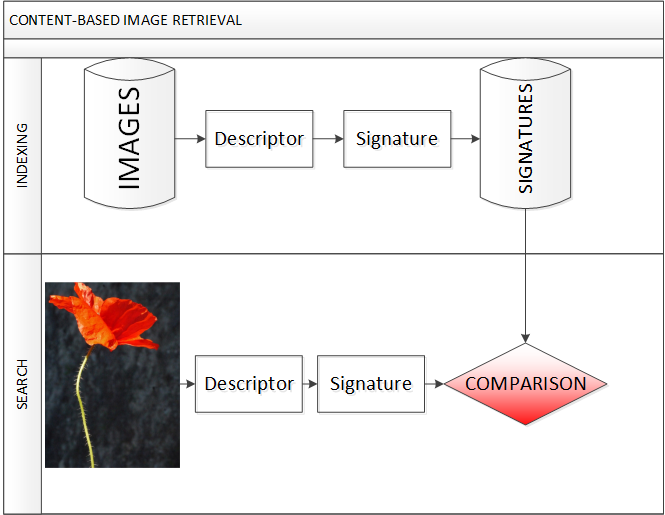
\includegraphics[height=2.5cm]{knnTopImg.png}};
\end{tikzpicture}

- Application for image classification

\begin{itemize}
\item More complex data.
\item Distances on signature vectors extracted from the K-mean method.
\item One most adapted distance type for each descriptor .
\end{itemize}

\end{frame}



\begin{frame} \frametitle{Results and Discussion (1/3)}

% Image en haut a droite rapellant l'avancee dans le process flow
\begin{tikzpicture}[remember picture, overlay]
  \node [anchor=north east, inner sep=2pt]  at (current page.north east)
     {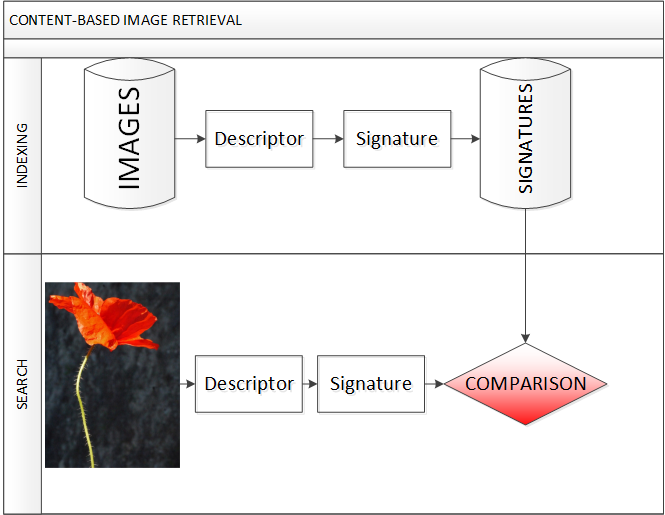
\includegraphics[height=2.5cm]{knnTopImg.png}};
\end{tikzpicture}

\begin{itemize}
\item Reduce data-base of 100 images composed of 4 species.
\end{itemize}

\begin{figure}[htbp]
\begin{minipage}[c]{.45\linewidth}
\begin{center}
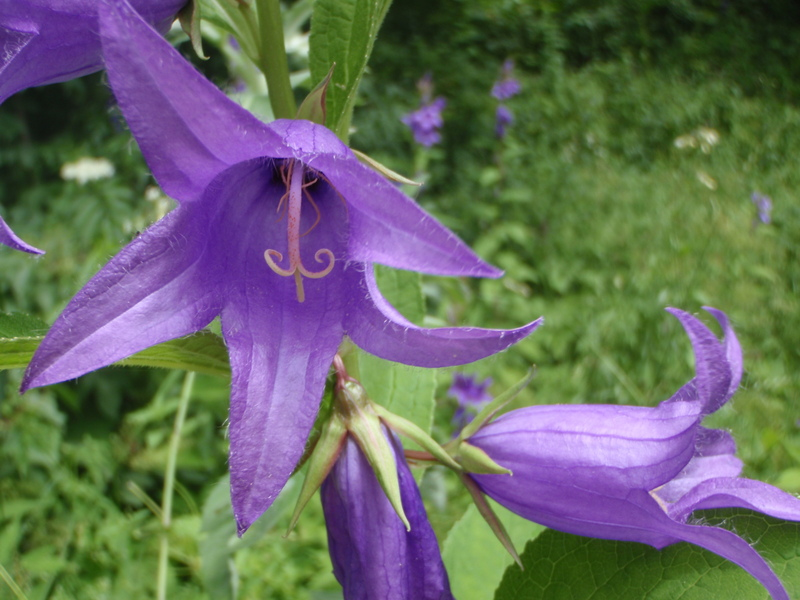
\includegraphics[scale=0.40]{63.jpg}
\caption{Specie Id: 173}
\label{fig:image4}
\end{center}
\end{minipage}
\hfill
\begin{minipage}[c]{.45\linewidth}
\begin{center}
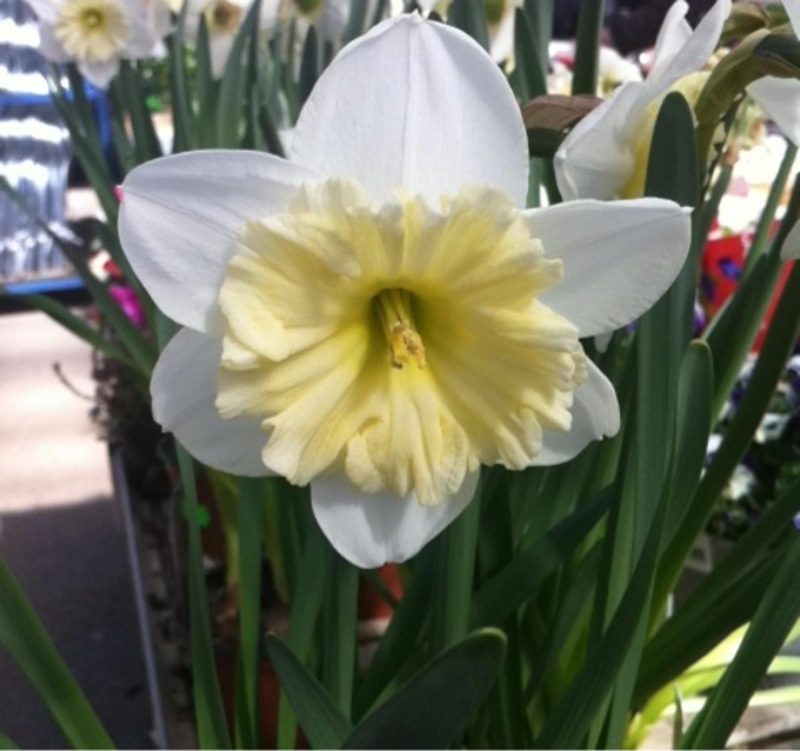
\includegraphics[scale=0.08]{2391.jpg}
\caption{Specie Id: 1102 }
\label{fig:image5}
\end{center}
\end{minipage}
\end{figure}


\begin{figure}[htbp]
\begin{minipage}[c]{.45\linewidth}
\begin{center}
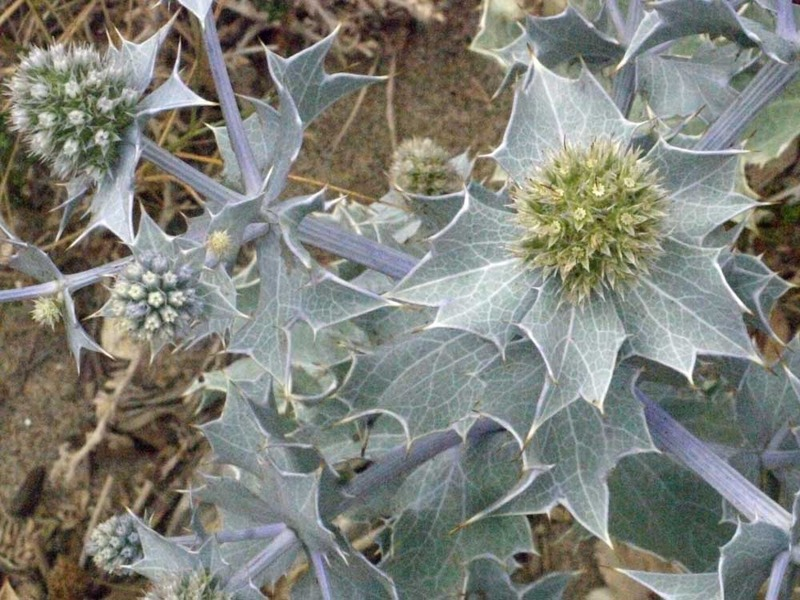
\includegraphics[scale=0.20]{4971.jpg}
\caption{Specie Id: 1889}
\label{fig:image6}
\end{center}
\end{minipage}
\hfill
\begin{minipage}[c]{.45\linewidth}
\begin{center}
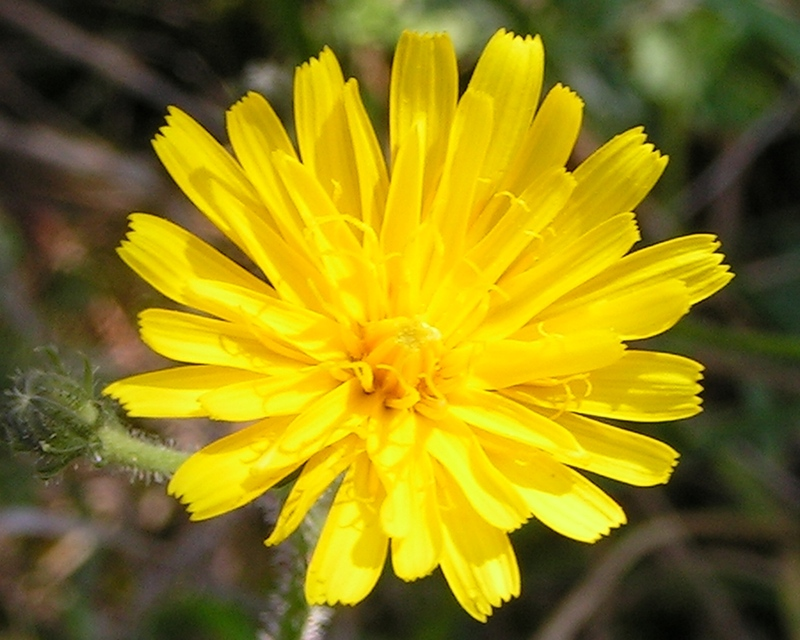
\includegraphics[scale=0.08]{21604.jpg}
\caption{Specie Id: 2717}
\label{fig:image7}
\end{center}
\end{minipage}
\end{figure}

\end{frame}


\begin{frame} \frametitle{Results and Discussion (2/3)}
%----------------------------------------------------------------------------------------

% Image en haut a droite rapellant l'avancee dans le process flow
\begin{tikzpicture}[remember picture, overlay]
  \node [anchor=north east, inner sep=2pt]  at (current page.north east)
     {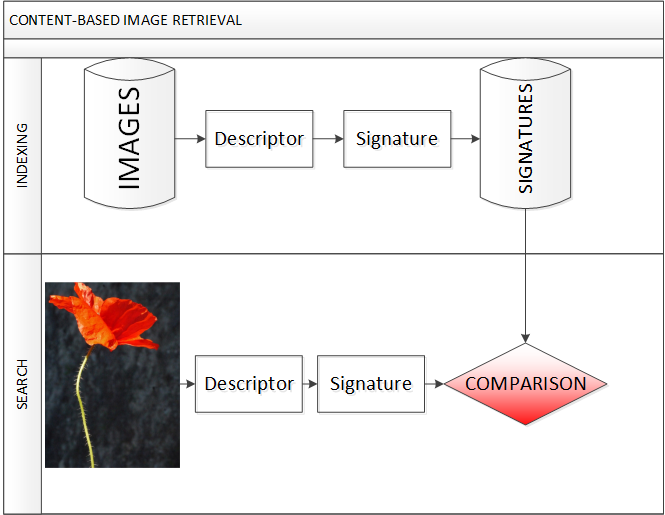
\includegraphics[height=2.5cm]{knnTopImg.png}};
\end{tikzpicture}

\begin{itemize}
\item Compare the two descriptors SIFT and C$_2$O.
\end{itemize}

\begin{tiny}
\begin{table}[H]
\centering
\caption{SIFT and C$_2$O results}
\label{tab1}
\begin{tabular}{|l|l|l|l|l||l|l|}
\hline
ID & Training Base & Test Base & Correct (SIFT) & Correct (C$_2$O) & Accuracy (SIFT) & Accuracy (C$_2$O) \\ \hline
173 & 17 & 8 & 4 & 1 & 50\% & 12.5\% \\ \hline
1102 & 22 & 3 & 1 & 1 & \cellcolor{red!75} 33\% &\cellcolor{red!75} 33\% \\ \hline
1889 & 16 & 9 & 1 & 0 & 11\% & 0\% \\ \hline
2717 & 15 & 10 & 7 & 7 &\cellcolor{red!75} 70\% &\cellcolor{red!75} 70\% \\ \hline
Total & 70 & 30 & 13 & 9 & / & / \\ \hline
\end{tabular}
\end{table}
\end{tiny}

\begin{itemize}
\item Classification
\vspace{0.3cm}
\begin{itemize}
\item To much reducing on the K-means (100 words).
\vspace{0.15cm}
\item Euclidean distance not the most efficient or adapt.
\end{itemize}
\end{itemize}

\end{frame}
%----------------------------------------------------------------------------------------

\begin{frame} \frametitle{Results and Discussion (3/3)}

% Image en haut a droite rapellant l'avancee dans le process flow
\begin{tikzpicture}[remember picture, overlay]
  \node [anchor=north east, inner sep=2pt]  at (current page.north east)
     {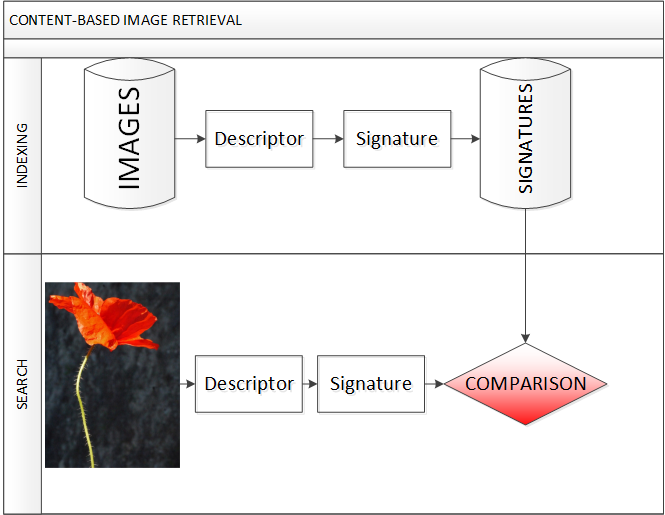
\includegraphics[height=2.5cm]{knnTopImg.png}};
\end{tikzpicture}


\begin{tiny}
\begin{table}[H]
\centering
\caption{SIFT and C$_2$O results}
\label{tab1}
\begin{tabular}{|l|l|l|l|l||l|l|}
\hline
ID & Training Base & Test Base & Correct (SIFT) & Correct (C$_2$O) & Accuracy (SIFT) & Accuracy (C$_2$O) \\ \hline
173 & 17 & 8 & 4 & 1 & 50\% & 12.5\% \\ \hline
1102 & 22 & 3 & 1 & 1 & \cellcolor{red!75} 33\% &\cellcolor{red!75} 33\% \\ \hline
1889 & 16 & 9 & 1 & 0 & 11\% & 0\% \\ \hline
2717 & 15 & 10 & 7 & 7 &\cellcolor{red!75} 70\% &\cellcolor{red!75} 70\% \\ \hline
Total & 70 & 30 & 13 & 9 & / & / \\ \hline
\end{tabular}
\end{table}
\end{tiny}

\begin{itemize}
\item C$_2$O
\vspace{0.3cm}
\begin{itemize}
\item The concatenation way is not optimal.
\item Parameters D, alpha, and beta has to be discussed regarding to the images.
\end{itemize}
\end{itemize}
\end{frame}
%----------------------------------------------------------------------------------------
%%-----------------------------------------------------------------------------------------
\section{Project management}
%%-----------------------------------------------------------------------------------------




\begin{frame} \frametitle{Scheduling (1/2)}
%%-----------------------------------------------------------------------------------------
% Montrer le passage d'un gantt a un backlog produit, => mettre l'accent sur la modification du gantt sans modification du backlog notable

\begin{itemize}
\item The forecast Gantt chart  :
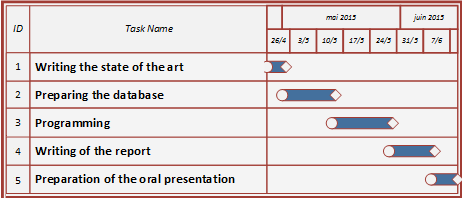
\includegraphics[scale=0.80]{GanttPrez.png}
\item All time affectation done before the beginning of the project
\item Rarely respected in important project
\end{itemize}

\end{frame}
%%-----------------------------------------------------------------------------------------


\begin{frame} \frametitle{Scheduling (2/2)}
%%-----------------------------------------------------------------------------------------
% Montrer le passage d'un gantt a un backlog produit, => mettre l'accent sur la modification du gantt sans modification du backlog notable


\begin{itemize}
\item The project backlog  :
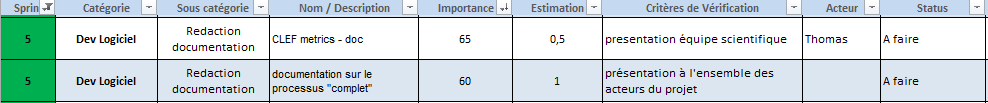
\includegraphics[scale=0.50]{backlog.png}
\item What is the backlog?
\item Advantages of the backlog
\item Drawbacks of the backlog
\end{itemize}


\end{frame}
%%-----------------------------------------------------------------------------------------




%%-----------------------------------------------------------------------------------------
\section{Conclusion}
%%-----------------------------------------------------------------------------------------

\begin{frame} \frametitle{Sum-up of the situation}
%%-----------------------------------------------------------------------------------------

\begin{columns}[t]
  \begin{column}{5cm}
  \begin{block}{Starting objectives}
	\begin{itemize}
		\item SIFT tests
		\item C$_2$O programming
		\item classification programming
		\item Code optimizing for speed
		\item parallelization
	\end{itemize}
  \end{block}
  \end{column}

  \begin{column}{5cm}
  \begin{block}{Ending situation}
  \begin{itemize}
		\item SIFT tests
		\item C$_2$O programming
		\item Classification programming
  \end{itemize}
  \end{block}
  \end{column}
 \end{columns}

\begin{alertblock}{Issues}
	\begin{itemize}
		\item C$_2$O concatenation order
		\item Distance calculation
	\end{itemize}	
\end{alertblock}
\end{frame}



\begin{frame}\frametitle{Personal conclusion}
%----------------------------------------------------------------------------------------
\begin{columns}[t]
  \begin{column}{5cm}
    \begin{block}{Personal gains}
      \begin{itemize}
            \item New way to organize teamwork
            \item Technical knowledge
            \item Contest participation context
            \item Code management on a project scale
      \end{itemize}
    \end{block}
  \end{column}

  \begin{column}{5cm}
  \begin{block}{Perspectives}
  \begin{itemize}
        \item Fixing technical issues
        \item Test on the whole database
  \end{itemize}
  \end{block}
  \end{column}
\end{columns}


\end{frame}


\section{}
\begin{frame}\frametitle{}
%%-----------------------------------------------------------------------------------------
    \begin{center}
        \huge Thank you for attention
    \end{center}
\end{frame}
%%-----------------------------------------------------------------------------------------


\end{document}

